\chapter{User Interfaces}

So far we have worked hard on the core mechanic of our game. Another important
aspect are the screens and components that wrap this mechanic. In this chapter
you will learn how to implement menus, popups and other user interface elements
in \cocos{}. 

\cocos{} provides its own set of basic UI components, such as buttons and
labels. For most games these components are sufficient. However, in this chapter
we also learn how to integrate Apple's UI framework \textit{UIKit}. Knowing
that is important for integrating many core Apple API's. As a specific example,
we will add integrate the Game Center framework in this chapter.

By the end of this chapter we will have a fully functional game!
Here's the basic screen flow our game will have:

\begin{figure}[H]
		\centering
		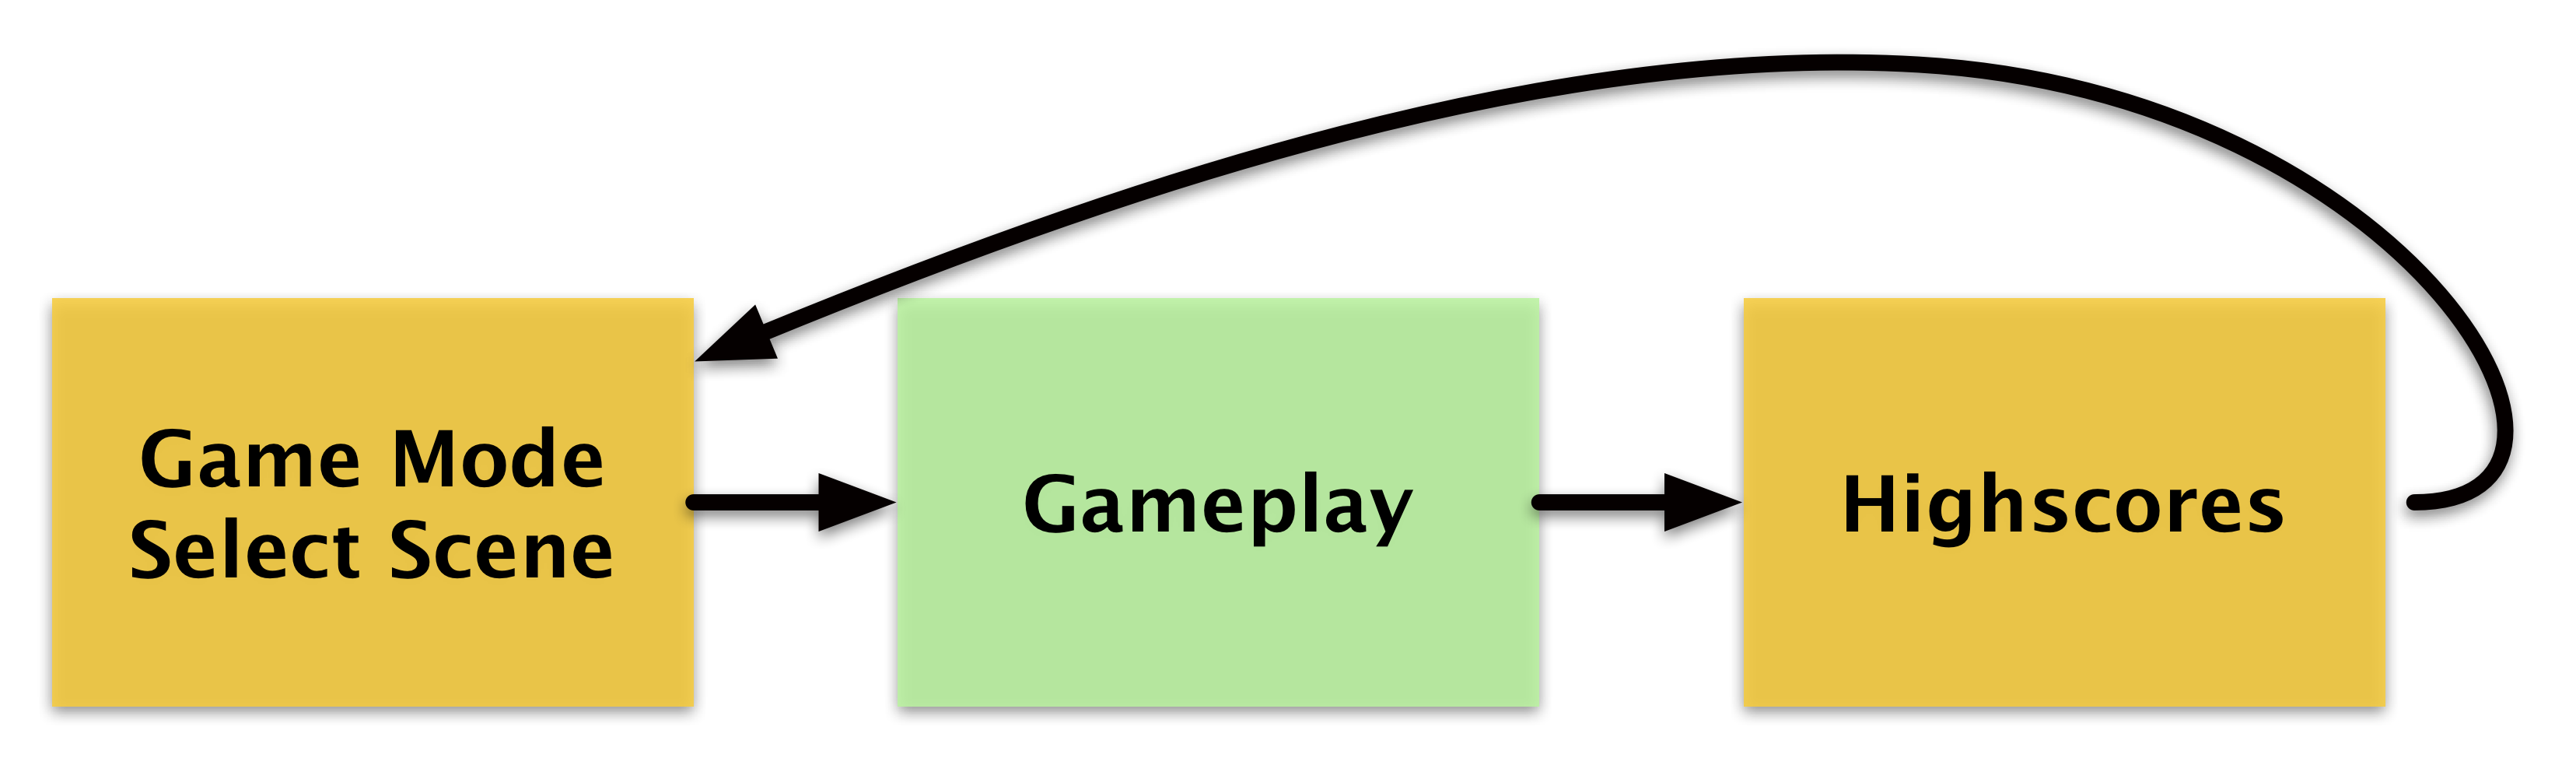
\includegraphics[width=0.7\linewidth]{images/Chapter6/screen_flow.png}
\end{figure}

Throughout this chapter you will not only learn how to build user interfaces
with \cocos{} and \SB{}, you will also learn how to structure this game to
support two different gameplay modes. We will implement and \textit{endless} and
a \textit{timed} gameplay mode, each with a different set of rules and
behaviors.

Let's start out by adding the game mode selection scene!

\section{Adding a game mode selection scene}
We will now change the screen flow of our existing game. Instead of diving into
the gameplay directly the user will see a game mode selection scene when
starting the game. 

The game mode selection scene will allow the user to swipe to switch between the
endless and timed game mode. Luckily \cocos{} provides a component called
\inlinecode{CCScrollView}\index{User Interface!CCScrollView} that implements
most of the functionality that we need for that scene.

\begin{leftbar}
Open the \SB{} project and create a new File (File -> New -> File\ldots). Name
the new file \textit{StartScene} and select \texit{Scene} as the type.
\end{leftbar}

We will create a game mode select scene that smoothly transitions into the
gameplay. To accomplish that we'll use the same background image for this scene
as for the actual gameplay. 

\begin{leftbar}
Drag the image \textit{backround.png} image onto the stage; it becomes the first
child of the root node of our new \textit{StartScene}.
\end{leftbar}

The background image should have exactly the same settings as in
\textit{MainScene} so that it fills the entire scene.

\begin{leftbar}
Select the background sprite in the timeline and apply the following steps:
\begin{enumerate}
  \item Set the position type for X to \textit{percentage of parent container}
  \item Set the X position to \textit{50}
  \item Set the position type for Y to \textit{percentage of parent container}
  \item Set the Y position to \textit{50}
\end{enumerate}
\end{leftbar}

Now the background image should fill the entire background. We will be
presenting some information in front of that background. To make that
information stand out more we will dim the background a little bit by turning
down its opacity. Since the fill color behind the background image is black a
lower opacity will result in a darker image.

\begin{leftbar}
Select the background sprite in the timeline. Set the opacity in the property
inspector to \textit{0.7}:
\begin{figure}[H]
		\centering
		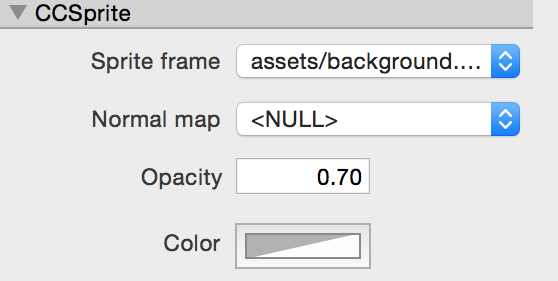
\includegraphics[width=200pt]{images/Chapter6/opacity_lower.png}
\end{figure}
\end{leftbar}

Next, we are going to add a label with an instruction for the player. A label is
a simple UI component that can display text. When building games with \cocos{}
we want to place the most UI components relative to screen edges. Using this
approach the UI will still look good when the game runs on a device with a
different screen size. Here's a little illustration:

\begin{figure}[H]
		\centering
		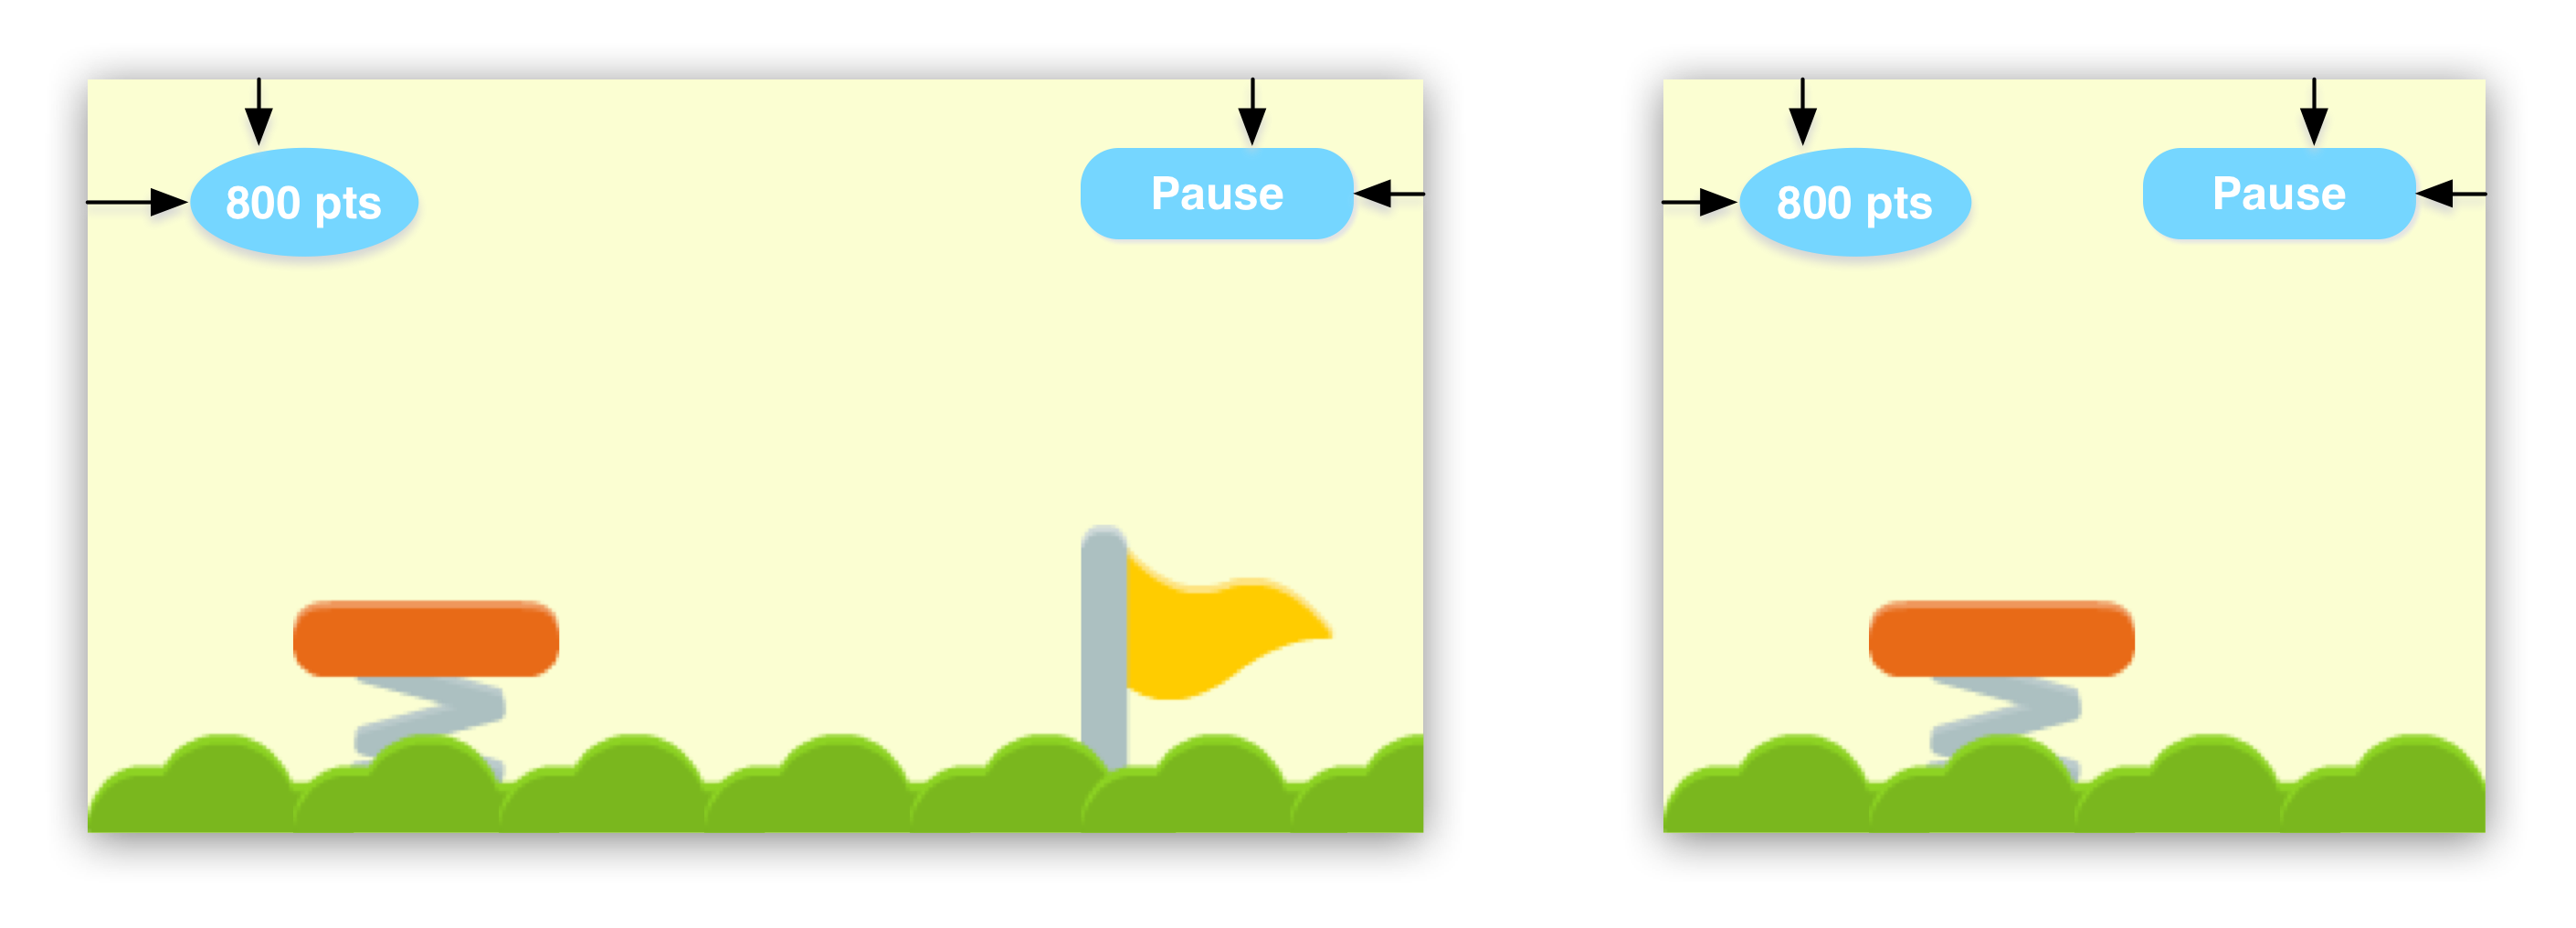
\includegraphics[width=0.7\linewidth]{images/Chapter6/multiple_screen_sizes.png}
		\caption{UI elements should be placed relative to screen edges to preserve
		their position on different screen sizes}
\end{figure}

Throughout this chapter we will use \cocos{}'s reference
corner feature to accomplish resizable user interfaces. 

\begin{leftbar}
Drag a \textit{CCLabelTTF} from the node library \textit{onto} the background
sprite, so that it becomes a child of it. Set the position up as following:
\begin{enumerate}
  \item Set the position to be relative from the \textit{Top-left}.
  \item Set the position type for X to \textit{percentage of parent container}
  \item Set the X position to \textit{50}
  \item Set the Y position to \textit{80}
\end{enumerate}

Set the label text to: \textit{Choose your game mode:}. We also want to change
the font and appearance of this label a little:
\begin{enumerate}
  \item As font name choose: \textit{Optima-Bold}
  \item As font size choose: \textit{40}
  \item Set the draw color to \textit{black}
  \item Set the outline color to \textit{white}
  \item Set the outline width to \textit{6}
\end{enumerate}
\end{leftbar}
